\chapter{Literature survey}

\section{Supervised Learning}

The machine learning model built using existing dataset is called supervised learning. ´Figure1 illustrates the supervised learning workflow. In this paper, author builds a supervised learning model to predict the product taxonomies. The work flow starts with data collection, this step involves fetching the corpus of raw data. This raw data processed before creating a training data set out of it. The data preprocessing steps involves feature selection, text normalization, data imputation and feature extraction. The training data is passed an input to the model which compares its results with the actual value to self- evaluate and learn. If any hyperparameter tuning for the machine learning model is required then it is trained again with new parameters. The model is then evaluated and then deployed for production use.
\begin{figure}[h!]
    \centering    
    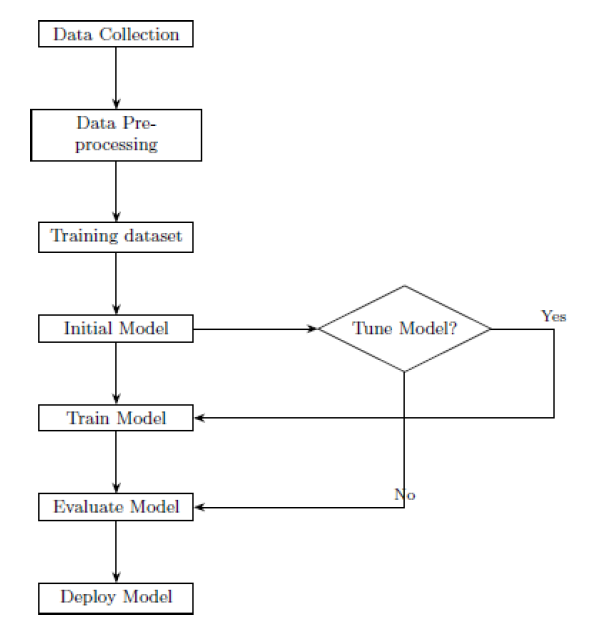
\includegraphics[scale=0.8]{supervised_learning.png}
    \caption{Supervised Learning}
\end{figure}


\section{Machine Learning Techniques in Traffic Prediction}

Machine learning techniques have shown great promise in traffic flow prediction due to their ability to learn from data and capture complex patterns. Key machine learning techniques explored in the literature include:

\begin{itemize}
    \item Linear Regression
    \item Decision Trees and Random Forest
    \item Support Vector Machines (SVM)
    \item Neural Networks
    \item Deep Learning Models (Recurrent Neural Networks (RNN), Long Short-Term Memory (LSTM))
 
    

\end{itemize}

\section{Comparative Studies}

Several comparative studies have evaluated the performance of different machine learning models in traffic flow prediction. These studies provide insights into the strengths and weaknesses of various models, guiding the selection of appropriate techniques for specific scenarios.



